\documentclass[]{article}
\usepackage[]{graphicx} 
\usepackage[utf8]{inputenc} 
\usepackage[OT1]{fontenc} 
\usepackage[]{subcaption} 
\usepackage{simplewick}
\usepackage{caption}
\usepackage{amsmath}
\usepackage[makeroom]{cancel}
\usepackage[]{mathtools} 
\usepackage[]{amssymb} 
\usepackage{prettyref}
\newrefformat{fig}{Figure~[\ref{#1}]}


\begin{document}

\title{Policy Gradient}
\author{Felipe Marcelino}
\date{21 May 2020}
\maketitle

\section{Notes}


\subsection*{Today's Lecture }%
\label{sub:Slide 3}

\begin{enumerate}
    \item The policy gradient algorithm
    \item What does the policy gradient do?
    \item Basic variance reduction: causality
    \item Basic variance reduction: baselines
    \item Policy gradient examples
    \item Goals:
        \begin{itemize}
            \item Understand policy gradient reinforcement learning
            \item Understand practical considerations for policy gradients
        \end{itemize}
\end{enumerate}

\subsection*{Evaluating the objective}%
\label{sub:Evaluating the objective}


\par The objective of RL that we would like to optimize: 

\begin{equation}
\label{eq:objective}
\theta_{*} = \underset{\theta}{\text{argmax}} \underbrace{E_{\tau \sim p_{\theta}(\tau)} \Big[
\sum_{t}r(s_{t},a_{t}}_{J(\theta)} \Big]
\end{equation}

Expanding $\pi_{\theta}$ results in:
\begin{equation}
    \label{eq:pitheta}
    \pi_{\theta}(s_1,a_1,\cdots,s_{T},a_{T}) = p(s_1) \prod_{t=1}^{T}\pi_{\theta}(a_{t}|s_{t})p(s_{t+1}|s_{t},a_{t})
\end{equation}

\par The following equations are finite and infinite horizon cases. 

\captionof*{figure}{Infinite Horizon Case}
\begin{equation}
    \theta_{*} = \underset{\text{argmax}}{\theta} E_{(s,a) \sim p_{\theta}(s,a)} [r(s,a)] 
\end{equation}

\captionof*{figure}{Finite Horizon Case}
\begin{equation}
    \theta_{*} = \underset{\text{argmax}}{\theta} \sum_{t=1}^{T}E_{(s,a) \sim p_{\theta}(s,a)} [r(s,a)]
\end{equation}

Now how it is possible to maximize the expectation of equation \eqref{eq:objective} under the trajectory distribution generated by the
policy $\pi_{\theta}$ ? Before answering the question above, let us try something more fundamental. How do we obtain the
estimate of this expected value without knowing the transition distribution and the initial state distribution? 
\begin{itemize}
    \item It is possible to generate samples from the distribution under which expectation is taken. Then
        calculate the average of the values of the quantity inside the expectation over those samples:
    \begin{equation}
        \label{eq:samples1}
        J(\theta) \approx \frac{1}{N} \sum_{i} \sum_{t} r(s_{i,t},a_{i,t})
    \end{equation}
\end{itemize}

\begin{figure}
\begin{center}
    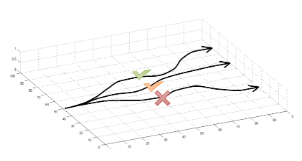
\includegraphics[scale=0.5]{cap4img/trajectories.png}
\end{center}
\caption{Trajectories: Calculate $J(\theta) $ summing the rewards of these trajectories.}
\label{fig:trajectories}
\end{figure}


\subsection*{Direct Policy Differentiation}
\label{sub:Direct Policy Differentation}

The following notation is another notation for $J(\theta)$ :
\begin{equation}
    \label{eq:jtheta}
    J(\theta) = E_{\tau \sim \pi_{\theta}(\tau)}\underbrace{[r(\tau)]}_{\sum_{t=1}^{T}r(s_{t},a_{t})} = \int
    \pi_{\theta}(\tau) r(\tau) d\tau
\end{equation}

\begin{equation}
    \label{eq:deltatheta}
    \triangledown_{\theta}J(\theta)= \int  \triangledown_{\theta}\pi_{\theta}(\tau) r(\tau) d\tau
\end{equation}

Now using the following identity: $\pi_{\theta}(\tau) \triangledown_{\theta}log\pi_{\theta}(\tau) =
\pi_{\theta}\frac{\triangledown \pi_{\theta}(\tau)}{\pi_{\theta}(\tau)} = \triangledown_{\theta} \pi_{\theta}(\tau)$,
to transform the equation \eqref{eq:deltatheta}:

\begin{equation}
    \label{eq:expecteddelta}
    \triangledown_{\theta}J(\theta) = \int
    \pi_{\theta}(\tau)\triangledown_{\theta}log\pi_{\theta}(\tau)r(\tau)d\tau = E_{\tau \sim
    \pi_{\theta}(\tau)}[\triangledown_{\theta}log\pi_{\theta}(\tau)r(\tau)]
\end{equation}

\par And now expanding $\pi_{\theta}$ as showed in equation \eqref{eq:pitheta} transform equation
\eqref{eq:expecteddelta} onto: 
\begin{equation}
    \triangledown_{\theta} \Big[ \cancel{logp(s_1)} + \sum_{t=1}^{T}log\pi_{\theta}(a_t|s_t) +
    \cancel{logp(s_{t+1}|s_t,a_t) }\Big]
\end{equation}
\captionof*{figure}{The two terms without $\theta$ is zero}

\begin{equation}
    \label{eq:thetajota}
    \triangledown_{\theta}J(\theta) = E_{\tau \sim \pi_{\theta}(\tau)} \bigg[
    \Big(\sum_{t=1}^{T}\triangledown_{\theta}log\pi_{\theta}(a_t|s_t)\Big)\Big(\sum_{t=1}^{T}r(s_t,a_t)\Big) \bigg]
\end{equation}

How to derivate equation \eqref{eq:thetajota}? It is possible to use the same idea from equation \eqref{eq:samples1}:
\begin{itemize}
    \item Generating samples throughout the policy iteration with the environment and evaluating trajectories
        rewards. Also, evaluate their $\triangledown_{\theta}log\pi_{\theta}$, multiply them by the rewards and average
        the result's multiplication.
        \begin{equation}
            \label{eq:samples2}
            \triangledown_{\theta}J(\theta) \approx
            \frac{1}{N}\sum_{i=1}^{N}\Big(\sum_{t=1}^{T}\triangledown_{\theta}log\pi_{\theta}(a_{i,t}|s_{i,t})\Big)\Big(\sum_{t=1}^{T}r(s_{i,t},a_{i,t})\Big)
        \end{equation}
\end{itemize}

\subsection*{Comparison to maximum likelihood}%
\label{sub:Comparison to maximum likelihood}
\begin{equation}
    \label{eq:maximum}
    \triangledown_{\theta}J_{ML}(\theta) \approx
    \frac{1}{N}\sum_{i=1}^{N}\Big(\sum_{t=1}^{T}\triangledown_{\theta}log\pi_{\theta}(a_{i,t}|s_{i,t})\Big)
\end{equation}

This is just supervised learning maximum likelihood.

\subsection*{Evaluating the policy gradient}%
\label{sub:Evaluating the policy gradient}

Finally, it is possible now to modify the parameters theta according to derivating of $J(\theta)$:
\begin{equation}
    \label{eq:update}
    \theta \leftarrow \theta + \alpha J(\theta)
\end{equation}

\begin{figure}
\begin{center}
    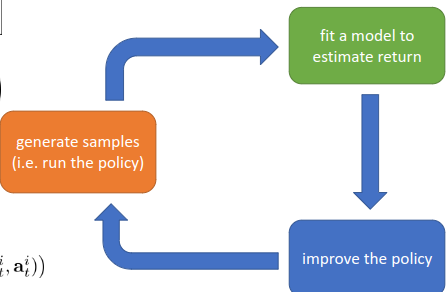
\includegraphics[scale=0.5]{cap4img/algorithm.png}
\end{center}
\caption{The algorithm consists of three parts: generation of samples,fit a model to estimate return and improve the
policy}
\label{fig:}
\end{figure}

REINFORCE algorithm:
\begin{enumerate}
    \item sample $\{\tau^{i}\}$ from $\pi_{\theta}(a_t|s_t)$ (run the policy)
    \item $\triangledown_{\theta}J(\theta) \approx
        \sum_{i}\big(\sum_{t}\triangledown_{\theta}log\pi_{\theta}(a_{t}^{t}|s_{t}^{i}a)\big)\big(\sum_{t}r(a_{t}^{i},a_{t}^{i})\big)$
    \item $ \theta \leftarrow \theta + \alpha J(\theta)$
\end{enumerate}
\begin{itemize}
    \item Doest not require the  initial state distribution or the transition probabilities. See equation \eqref{eq:samples2}
    \item Can be used in POMDP(Partially observed MDP) since Markov property is not use.
\end{itemize}


\subsection*{What did we just do?}%
\label{sub:What did we just do?}

\begin{equation}
    \label{eq:simpler}
    \triangledown_{\theta}J(\theta) \approx \frac{1}{N}\sum_{i=1}^{N}\triangledown_{\theta} log\pi_{\theta}(\tau_{i})
    r(\tau_{i})
\end{equation}
Equation \eqref{eq:simpler} is a cleaner version of equation \eqref{eq:samples2}.  It will take the take gradient of
$log\pi_{\theta}(\tau)$ that  points in the direction of trajectory $\tau$ and increase the probability of this
trajectory -- multiplying the $\tau$ trajectories by reward makes the high-reward trajectories more probable and the
lower reward trajectories less probable. Compared to the maximum likelihood gradient that makes everything more probable,
equation \eqref{eq:simpler}, on the other hand, penalize trajectories with bad reward expectation.


\subsection*{What is wrong with the policy gradient?}%
\label{sub:What is wrong with the policy gradient?}

\begin{itemize}
    \item  High Variance - When the policy gradient gets different samples, it get very different gradients from
        these samples. The gradient becomes very noisy, taking zig zag path and then the algorithm cannot converge.
\end{itemize}


\subsection*{Reducing Variance}%
\label{sub:Reducing Variance}

\par The first effort to reduce variance exploits the fact that the universe has causality. The past influences the
future, but not otherwise.
\begin{itemize}
    \item \textit{Causality}: policy at time \textit{t'} cannot affect reward at time \textit{t} when t $\leq$
        \textit{t'}
\end{itemize}

\begin{equation}
    \label{eq:reducingvariance}
    \nabla_{\theta} J(\theta) \approx \frac{1}{N} \sum_{i=1}^{N} \sum_{t=1}^{T} \nabla_{\theta} \log
\pi_{\theta}\left(\mathbf{a}_{i, t} | \mathbf{s}_{i, t}\right)\left(\sum_{\left.t^{\prime} = t\right.}^{T}
    r\left(\mathbf{s}_{i, t^{\prime}}, \mathbf{a}_{i, t^{\prime}}\right)\right) 
\end{equation}


Equation \eqref{eq:reducingvariance} states that the action choosing now $t^{\prime}$ will not affect the past rewards.
Take a look into the third $\sum$ and the subscript term. Consequently, the result of the multiplications of equation
\eqref{eq:reducingvariance} is going to be smaller than \eqref{eq:samples2}. Now, operations containing small numbers
are going to have a smaller variance. 

\begin{equation}\nabla_{\theta} J(\theta) \approx \frac{1}{N} \sum_{i=1}^{N} \sum_{t=1}^{T} \nabla_{\theta} \log \pi_{\theta}\left(\mathbf{a}_{i, t} | \mathbf{s}_{i, t}\right) \hat{Q}_{i, t}\end{equation}
\captionof*{figure}{$\hat{Q}$ = rewards to go}

\subsection*{Baselines}%
\label{sub:Baselines}

Another problem with the reward function is the rewards can be a larger number and the values next to each other. For
instance, if the rewards are between 999999 and 10000001, according to equation \eqref{eq:simpler}, they will be very
probably. Because of this, the gradient does not have good separation for the real good one's trajectories. Solution:
Adding a term \textit{b} that is: $b = \frac{1}{N}\sum_{i=1}^{N}r(\tau)$

\begin{equation}\nabla_{\theta} J(\theta) \approx \frac{1}{N} \sum_{i=1}^{N} \nabla_{\theta} \log \pi_{\theta}(\tau)[r(\tau)-b]\end{equation} 

The term \textit{b} helps the gradient. The good trajectories become most likely than the bad ones. This term is the
average reward of the samples. So \textit{b} increases the probability of the trajectories that is better than the
average and decreases probability of trajectories that is worst than the average.  The expectation $\left.E | \nabla_{\theta} \log \pi_{\theta}(\tau) b\right]$ is going to be
the same value that the expectation has before, but with less variance. Proof that the term \textit{b} does not affect
the expectation:

\begin{gather}
    E\left[\nabla_{\theta} \log \pi_{\theta}(\tau) b\right]=\int \pi_{\theta}(\tau) \nabla_{\theta}    \log\pi_{\theta}(\tau) b d \tau \\
    \int \nabla_{\theta} \pi_{\theta}(\tau) b d \tau=b \nabla_{\theta} \int \pi_{\theta}(\tau) d \tau \text{ (Integral of
    all probabilities is one)} \\
    b\nabla_{\theta}1 = 0
\end{gather}

The identity:  $\pi_{\theta}(\tau) \nabla_{\theta} \log \pi_{\theta}(\tau)=\nabla_{\theta} \pi_{\theta}(\tau)$,
transform right side of the equation (18) into equation left side of the equation (19). These proof affirms that it is
possible to subtract any constant into expectation, and the expectation will not change.

\par 
The optimal baseline is better than average baseline, but for implementation, average baseline are good enough: 
\begin{equation}b=\frac{E\left[g(\tau)^{2} r(\tau)\right]}{E\left[g(\tau)^{2}\right]}\end{equation}
The optimal baseline is the expected reward weighted by gradient magnitudes.
Proof: 
\begin{align*}
\text{Var}(x) &= E(x^2) - E(x)^2 \\
&= E _ { \tau \sim \pi _ { \theta } ( \tau ) } \left[ \big( \nabla _ { \theta } \log \pi _ { \theta } ( \tau ) ( r ( \tau ) - b ) \big) ^ { 2 } \right] - E _ { \tau \sim \pi _ { \theta } ( \tau ) } \left[ \nabla _ { \theta } \log \pi _ { \theta } ( \tau ) ( r ( \tau ) - b ) \right] ^ { 2 } \\
&= E _ { \tau \sim \pi _ { \theta } ( \tau ) } \left[ \big( \nabla _ { \theta } \log \pi _ { \theta } ( \tau ) ( r (
\tau ) - b ) \big) ^ { 2 } \right] - \cancel{\underbrace{E _ { \tau \sim \pi _ { \theta } ( \tau ) } \left[ \nabla _ { \theta } \log
\pi _ { \theta } ( \tau ) r ( \tau ) \right] ^ { 2 }}_{\text{this bit is just} E_{\tau \sim
\pi_{\theta}(\tau)}[\nabla_{\theta}log\pi_{\theta}(\tau)r(\tau)]}}
\end{align*}

Since \textit{b} is unbiased, the second term can be ignored. 
\par Let $g(\tau) = \nabla_{\theta}log\pi_{\theta}(\tau)$, compute the derivate of variance
with respect to \textit{b}.

\begin{align*}
\frac { d \text{Var} } { d b } &= \frac { d } { d b } E \left[ g ( \tau ) ^ { 2 } ( r ( \tau ) - b ) ^ { 2 } \right] \\
& = \frac { d } { d b } \left( E \left[ g ( \tau ) ^ { 2 } r ( \tau ) ^ { 2 } \right] - 2 E \left[ g ( \tau ) ^ { 2 } r ( \tau ) b \right] + b ^ { 2 } E \left[ g ( \tau ) ^ { 2 } \right] \right) \\
& = - 2 E \left[ g ( \tau ) ^ { 2 } r ( \tau ) \right] + 2 b E \left[ g ( \tau ) ^ { 2 } \right] = 0
\end{align*}

\par Solve the optimal value for \textit{b}:
\begin{equation}b=\frac{E\left[g(\tau)^{2} r(\tau)\right]}{E\left[g(\tau)^{2}\right]}\end{equation}


\subsection*{Policy Gradient is on-policy}%
\label{sub:Policy Gradient is on-policy}

On-policy definition: Every time the policy changes, it is necessary to generate new samples in order to improve the
policy.

$\nabla_{\theta} J(\theta)=\underbrace{E_{\tau \sim \pi_{\theta}(\tau)}}_{\text{This is trouble ...}}\left[\nabla_{\theta} \log \pi_{\theta}(\tau)
r(\tau)\right]$

What does it mean?

REINFORCE algorithm:
\begin{enumerate}
    \item sample $\{\tau^{i}\}$ from $\pi_{\theta}(a_t|s_t)$ (run the policy) $\leftarrow$ \textbf{THIS STEP CAN'T BE
        SKIPPED} 
    \item $\triangledown_{\theta}J(\theta) \approx
        \sum_{i}\big(\sum_{t}\triangledown_{\theta}log\pi_{\theta}(a_{t}^{t}|s_{t}^{i}a)\big)\big(\sum_{t}r(a_{t}^{i},a_{t}^{i})\big)$
    \item $ \theta \leftarrow \theta + \alpha J(\theta)$
\end{enumerate}

\begin{itemize}
    \item Neural networks change only a little bit with each gradient step. For this reason, it is necessary a large
        number of gradient steps
    \item On-policy learning can be extremely inefficient!
\end{itemize}

\subsection*{Off-policy learning \& importance sampling}
\label{sub:Off-policy learning importance sampling}

\subsubsection*{Importance Sampling:}
\label{sub:Importance Sampling}

\par Importance sampling is a technique to estimate the expectation of one distribution using a different
distribution.

\captionof*{picture}{Importance sampling}
\begin{equation}\begin{aligned}
E_{x \sim p(x)}[f(x)] &=\int p(x) f(x) d x \\
&=\int \frac{q(x)}{q(x)} p(x) f(x) d x \\
&=\int q(x) \frac{p(x)}{q(x)} f(x) d x \\
&=E_{x \sim q(x)}\left[\frac{p(x)}{q(x)} f(x)\right]
\end{aligned}\end{equation}

Plugging it into policy gradient
\begin{equation}J(\theta)=E_{\tau \sim \bar{\pi}(\tau)}\left[\frac{\pi_{\theta}(\tau)}{\bar{\pi}(\tau)} r(\tau)\right]\end{equation}

\par In that case, the samples come from $\vec{\pi}$ because we do not have samples from $\pi.$ As a result, the
policy becomes off-policy.

\begin{equation}
    \label{eq:sampling}
    \frac{\pi_{\theta}(\tau)}{\bar{\pi}(\tau)}=\frac{p\left(\mathbf{s}_{1}\right) \prod_{t=1}^{T}
\pi_{\theta}\left(\mathbf{a}_{t} | \mathbf{s}_{t}\right) p\left(\mathbf{s}_{t+1} | \mathbf{s}_{t},
\mathbf{a}_{t}\right)}{p\left(\mathbf{s}_{1}\right) \prod_{t=1}^{T} \bar{\pi}\left(\mathbf{a}_{t} | \mathbf{s}_{t}\right) p\left(\mathbf{s}_{t+1}+\mathbf{s}_{t}, \mathbf{a}_{t}\right)}=\frac{\prod_{t=1}^{T} \pi_{\theta}\left(\mathbf{a}_{t} | \mathbf{s}_{t}\right)}{\prod_{t=1}^{T} \bar{\pi}\left(\mathbf{a}_{t} | \mathbf{s}_{t}\right)}
\end{equation}

\par Equation \eqref{eq:sampling} states that only the action probability of the old and new policy is necessary for
calculating the expectation. 

\subsection*{The off-policy policy gradient}%
\label{sub:The off-policy  gradient}


\begin{equation*}\begin{aligned}
\nabla_{\theta^{\prime}} J\left(\theta^{\prime}\right) &=E_{\tau \sim \pi_{\theta}(\tau)}\left[\frac{\pi_{\theta^{\prime}}(\tau)}{\pi_{\theta}(\tau)} \nabla_{\theta^{\prime}} \log \pi_{\theta^{\prime}}(\tau) r(\tau)\right] \quad \text { when } \theta \neq \theta^{\prime} \\
&=E_{\tau \sim \pi_{\theta}(\tau)}\left[\left(\prod_{t=1}^{T} \frac{\pi_{\theta^{\prime}}\left(\mathbf{a}_{t} | \mathbf{s}_{t}\right)}{\pi_{\theta}\left(\mathbf{a}_{t} | \mathbf{s}_{t}\right)}\right)\left(\sum_{t=1}^{T} \nabla_{\theta^{\prime}} \log \pi_{\theta^{\prime}}\left(\mathbf{a}_{t} | \mathbf{s}_{t}\right)\right)\left(\sum_{t=1}^{T} r\left(\mathbf{s}_{t}, \mathbf{a}_{t}\right)\right)\right]
\end{aligned}\end{equation*}

The problem with the equation above is that if T is too large, the numbers will be enormous or too small.Consequently,
it causes the problem of increasing the variance of the expectation, and the all effort using the baseline is useless.
To solve this, we are going to use the first-order approximation for importance sampling.

\begin{equation*}\text { on-policy policy gradient: } \quad \nabla_{\theta} J(\theta) \approx \frac{1}{N} \sum^{N}
\sum^{T} \nabla_{\theta} \log \pi_{\theta}\left(\mathbf{a}_{i, t} | \mathbf{s}_{i, t}\right) \hat{Q}_{i,
t}\end{equation*}

\begin{equation*}\text { off-policy policy gradient: } \nabla_{\theta^{\prime}} J\left(\theta^{\prime}\right) \approx
\frac{1}{N} \sum_{i=1}^{N} \sum_{t=1}^{T} \frac{\pi_{\theta^{\prime}}\left(\mathbf{s}_{i, t}, \mathbf{a}_{i,
t}\right)}{\pi_{\theta}\left(\mathbf{s}_{i, t}, \mathbf{a}_{i, t}\right)} \nabla_{\theta^{\prime}} \log
\pi_{\theta^{\prime}}\left(\mathbf{a}_{i, t} | \mathbf{s}_{i, t}\right) \hat{Q}_{i, t}\end{equation*}


\begin{equation}\frac{1}{N} \sum_{i=1}^{N} \sum_{t=1}^{T} \underbrace{\cancel{\frac{\pi_{\theta^{\prime}}\left(\mathbf{s}_{i,
t}\right)}{\pi_{\theta}\left(\mathbf{s}_{i, t}\right)}}}_{\text{Ignore this part}} \frac{\pi_{\theta^{\prime}}\left(\mathbf{a}_{i, t} | \mathbf{s}_{i, t}\right)}{\pi_{\theta}\left(\mathbf{a}_{i, t} | \mathbf{s}_{i, t}\right)} \nabla_{\theta^{\prime}} \log \pi_{\theta^{\prime}}\left(\mathbf{a}_{i, t} | \mathbf{s}_{i, t}\right) \hat{Q}_{i, t}\end{equation}

\par The marginal distribution can be ignored, and policy is going to continue to improve \textbf{IF} $\theta^{\prime}$
is close to $\theta$. 

\subsection*{Policy gradient in practice}%
\label{sub:Policy gradient in practice}



\begin{itemize}
    \item Using much larger batches will help reducing variance.
    \item Tweaking learning rates is very hard. Adaptive step size rules like ADAM is okay.
\end{itemize}

\end{document}
